\documentclass[10pt]{article}

\usepackage{fullpage}
\usepackage{graphicx}
\usepackage{graphics}
\usepackage{mdwlist}
\usepackage[top=2.5cm, bottom=2.5cm, left=2.5cm, right=2.5cm]{geometry}
\usepackage{kotex}

\setlength{\oddsidemargin}{0.0in}
\setlength{\evensidemargin}{0.0in}
\setlength{\textwidth}{6.5in}
\setlength{\headheight}{0.0in}
\setlength{\topmargin}{0.0in}
% \setlength{\textheight}{9.0in}
\setlength{\textheight}{9in}
\addtolength{\textheight}{-\topmargin}
\addtolength{\textheight}{-\headheight}
\addtolength{\textheight}{-\headsep}
\addtolength{\textheight}{-\footskip}

\begin{document}

\newcommand{\beq}{\begin{equation}}
\newcommand{\eeq}{\end{equation}}
\newcommand{\bit}{\begin{itemize*}}
\newcommand{\eit}{\end{itemize*}}
\newcommand{\goal}[1]{ {\noindent {$\Rightarrow$} \em {#1} } }
\newcommand{\hide}[1]{}
\newcommand{\comment}[1]{ {\footnotesize {#1} } }
\newtheorem{lemma}{Lemma}
\newtheorem{theorem}{Theorem}
\newtheorem{proof}{Proof}
\newtheorem{defn}{Definition}
\newtheorem{algo}{Algorithm}
\newtheorem{observation}{Observation}

\title{Online Tensor Analysis}

\author{ {\em Sangjun Son} \\
	    Computer Science and Engineering \\
	    Seoul National University\\
	    {\tt lucetre@snu.ac.kr}
	 \and
	 {\em U Kang} \\
	    Computer Science and Engineering \\
	    Seoul National University\\
	     {\tt ukang@snu.ac.kr}
        }


\maketitle
\begin{abstract}
    
In this paper, we propose fast and accurate online tensor decomposition method called {\em OnlineTensorAnalysis}, which performs splitting its tensor and create a new factorization when drastic data change detection.

\end{abstract}

\section{Introduction}
    \label{sec:intro}
    
Given a temporally growing tensor, how can we analyze it efficiently? Multi-dimensional arrays or tensors have been widely used to model real world data. Tensor decomposition plays a significant role in latent feature discovery and estimation of unobservable entries. Each tensor can be classified as static or dynamic. A tensor whose size and values are temporally changing is dynamic (e.g. sensor data on every point of the room), and the other is static. Most of existing tensor analysis methods such as \cpals and \hosvd decompose static tensors with high fitness.

Data stream produces numerous amounts of data every second and it became more important to maintain tensor factorization result. Every dynamic tensor can have an extra temporal mode and previous state of the tensor can be stored along the mode. Growing in the temporal mode, however, applying static tensor factorization methods to dynamic is an inappropriate way in time and space efficiency. It invokes lots of computations to update all the entries of time factor matrix. The contributions of this project are the following:
\bit
\item \method performs online tensor decomposition preserving accuracy without time dilation due to short data income intervals.
\item \method is time scalable, being linear on the length of temporal mode. 
\item \method automatically detects drastic data changes and creates new starting point of decomposition.
\eit

\section{Preliminaries}
    \label{sec:prelim}
    \input{020prelim}
    
\newpage
\section{Proposed Method}
    \label{sec:proposed}
  	
We've developed our methods by extending the basic intuition of \ocp. Since dynamic tensor decomposition pursues shorter time factor updates, this results low accuracy factorization when real-time data incomes. To optimize the speed accuracy problem, we'd like to trigger static decomposition method, \cpals while dynamic method like \ocp is being done.

\begin{center}
	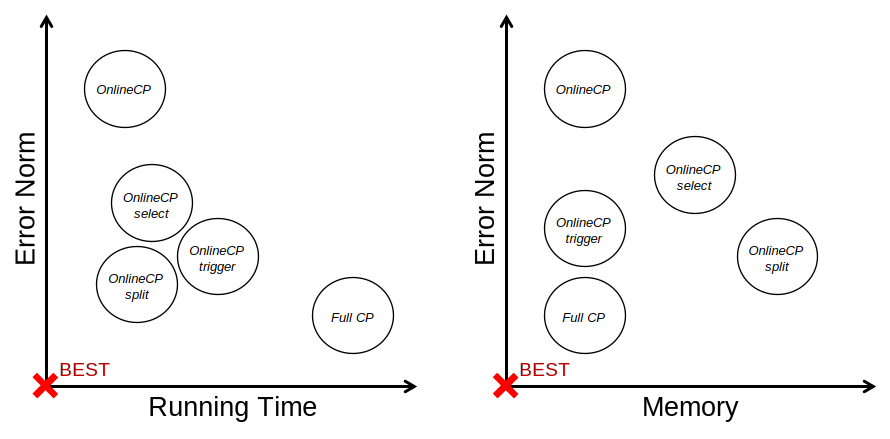
\includegraphics[width=1\textwidth]{FIG/Method-optimization.pdf}
\end{center}

\newpage
\subsection{\em OnlineCP-trigger}
\textbf{Detection Approach}: \cpals activates whole temporal factor updates and enables high accuracy decomposition. Drastic data can be detected by calculating image error norm and its ratio between neighboring time steps. The moment for triggering \cpals is when temporal ratio of error norm for incoming data exceeds threshold ${\theta}_{update}$.

\begin{align*}
%    \theta < \frac{\norm{\tilde{\chi}_{i}-\chi_{i}}}{\norm{\tilde{\chi}_{i-1}-\chi_{i-1}}}
    {\theta}_{update} < \norm{\tilde{\chi}_{i}-\chi_{i}}-\norm{\tilde{\chi}_{i-1}-\chi_{i-1}} 
\end{align*}

\begin{center}
	\includegraphics[width=0.85\textwidth]{FIG/OnlineCP-trigger.png}
\end{center}

\newpage
\subsection{\em OnlineCP-split}
\textbf{Split Approach}: trigger function in detection approach tells us sudden change in data. What if the incoming data may have a new theme unseen before? It implies that new decomposition starting point with tensor split is needed. In this approach, we'd like to apply the trigger function for splitting the tensor into serial tensors of different themes. (e.g. $A$, $B$, $C$, $D$)

\begin{center}
	\includegraphics[width=0.9\textwidth]{FIG/OnlineCP-split.png}
\end{center}

\newpage
\subsection{\em OnlineCP-select}
\textbf{Selection Approach}: Similarly to split approach, trigger function now decides whether to split or to concatenate behind after one temporal factor update. It allows to store the tensor efficiently by grouping tensors with similar themes and splitting them otherwise. (e.g. $A$, $B$, $B'$, $C$)

\begin{align*}
    {\theta}_{update} < \norm{\tilde{\chi}_{i}-\chi_{i}}-\norm{\tilde{\chi}_{i-1}-\chi_{i-1}} <{\theta}_{split} \\
    \norm{\tilde{\chi}_{i}-\chi_{i}}-\norm{\tilde{\chi}_{i-1}-\chi_{i-1}} \geqslant {\theta}_{split}
\end{align*}

\begin{center}
	\includegraphics[width=0.9\textwidth]{FIG/OnlineCP-select.png}
\end{center}


\section{Experiments}
    \label{sec:experiments}
    

\subsection{\em Dataset}
We've constructed synthetic data to manually make temporally changing points. A tensor has its size of $10*20*30*1000$ having the last mode as a temporal mode. The tensor $\chi$ was conducted by concatenation of theme tensor $T$ which is addition of three tensors $T_{main}$, $T_{theme}$ and $T_{noise}$. Each consisting tensor is 100x, 10x and 1x normal distributed randomized tensor respectively and those are used for making different and similar theme tensors.

\begin{table}[htb]
\small
\begin{tabular}{ c | cccccccccc }
 \hline
 Time Index & 1$\sim$100 & 101$\sim$200 & 201$\sim$250 & 251$\sim$500 & 501$\sim$600 & 601$\sim$700 & 701$\sim$750 & 751$\sim$800 & 801$\sim$950 & 951$\sim$1000 \\
 \hline
 Theme & $A$ & $A'$ & $B$ & $B'$ & $B''$ & $C$ & $D$ & $E$ & $E'$ & $E''$ \\
 \hline
\end{tabular}
\end{table}

\subsection{\em Experimental Setting}
In the experiment, we've set rank as 10, temporal batch size as 1 and initial size for \ocp as 5.
 
\begin{center}
	\includegraphics[width=1\textwidth]{FIG/Comparison-analysis.pdf}
\end{center}

    
\section{Related Works}
    \label{sec:related}
    \input{050related}    

\section{Conclusions}
    \label{sec:conclusions}
    \input{060conclusions}


\bibliography{BIB/other}
\bibliographystyle{plain}

\newpage
\appendix
\section{Appendix}

\subsection{Additional Stuff 1}
Put contents here.

\subsection{Additional Stuff 2}
Put contents here.


\end{document}
